\documentclass[aspectratio=169]{beamer}
\usetheme{Madrid}
\usecolortheme{beaver}
\usepackage[utf8]{inputenc}
\usepackage[T1]{fontenc}
\usepackage{tikz}
\usepackage{amssymb}
\usepackage{graphicx}
\setbeamertemplate{navigation symbols}{}
\setbeamercolor{title}{fg=white,bg=cyan!60!black}
\setbeamercolor{frametitle}{fg=white,bg=cyan!50!black}
\setbeamercolor{block title}{bg=cyan!15,fg=black}
\setbeamercolor{block body}{bg=cyan!5,fg=black}

\title{Story Studio 1 — Page Basics}
\subtitle{Lesson 1: Front Page}
\author{ByteForge --- Grade 7 --- Game Maker}
\date{}

\begin{document}

\begin{frame}
    \titlepage
\end{frame}

\begin{frame}{A heading is a page's title}
    \Large
    One big title, shown once near the top — the ONE thing that tells a reader what this whole page is about. This is what a real webpage's \texttt{<h1>} does.

    \begin{center}
    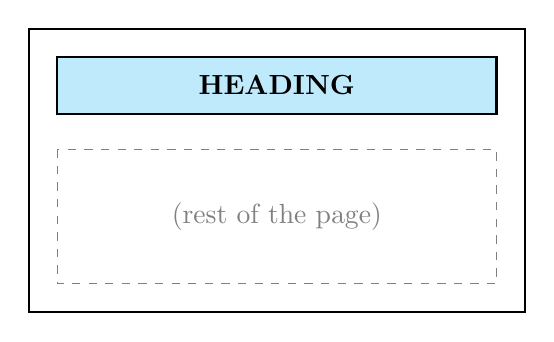
\begin{tikzpicture}[scale=0.9]

        \draw[thick] (0,0) rectangle (7,-4);
        \draw[fill=cyan!25, thick] (0.4,-0.4) rectangle (6.6,-1.2);
        \node at (3.5,-0.8) {\bfseries HEADING};
        \draw[dashed, gray] (0.4,-1.7) rectangle (6.6,-3.6);
        \node[gray] at (3.5,-2.65) {(rest of the page)};
    \end{tikzpicture}
    \end{center}
\end{frame}

\begin{frame}{A heading is a page's title --- Worked Example}
    \Large
    Worked example: a page with TWO heading blocks reads like a book with two titles on the cover — which one is it actually about? That's why real pages almost always use exactly one.
\end{frame}

\begin{frame}{Your Turn}
    \Large
    Open the student map, find \textbf{Story Studio 1 — Page Basics}, and complete
    the \textbf{Front Page} challenge --- everything you just saw, they now do themselves.
\end{frame}

\end{document}
